\documentclass[a4paper,10pt]{book}

\usepackage{xcolor}
\usepackage{tcolorbox}

\usepackage{geometry}
\geometry{
    right=1cm,
    left=1cm,
    top=2cm,
    bottom=2cm
}

\usepackage{tikz}
\usepackage{dblfnote}
\usepackage{lipsum}

\usepackage{xepersian}
\settextfont{Vazirmatn-Regular.ttf}

\newtcolorbox{ScientificDefinition}[1][]{
    colback=black!5,
    colframe=black!30,
    title=تعریف علمی
}

\title{\Huge جزوه الگوریتم‌های گراف}
\author{استاد مربوطه:\\سرکار خانم دکتر معصومه دامرودی}
\date{نویسنده:\\محمد خورشیدی روزبهانی}

\linespread{1.5}

\begin{document}

    \maketitle

    سلام

    \tableofcontents

    \chapter{مقدمات}

        در دنیای امروزی پر از فناوری و ارتباطات، مفاهیمی مانند گراف‌ها به عنوان ابزارهای بسیار قدرتمندی در حل مسائل گوناگون مورد استفاده قرار می‌گیرند. گراف‌ها، نه تنها در علوم کامپیوتر بلکه در زمینه‌های مختلفی از جمله شبکه‌های اجتماعی، حمل و نقل، مهندسی، و بیولوژی نیز کاربرد دارند.

        مسئله اویلر
        \footnote{\hspace{2pt}Euler}
        و پل کونیگزبرگ
        \footnote{\hspace{2pt}bridges Koningsberg}
        به عنوان یکی از مسائل کلاسیک و جذاب در تئوری گراف مطرح است که تاریخچه طولانی‌اش به اوایل قرن هجدهم بازمی‌گردد. این مسئله ابتدا توسط ریاضی‌دان معروف لئونارد اویلر
        \footnote{\hspace{2pt}Euler Leonhard}
        مطرح شد و بعدها توسط رابرت لویس کونیگزبرگ
        \footnote{\hspace{2pt}Konigsberg Louis Robert}
        مورد تحقیق و توسعه قرار گرفت.

        پل کونیگزبرگ، یکی از شهرهای کوچک در استان پروسیا
        \footnote{\hspace{2pt}Prussia of Province}
        (اکنون بخشی از شهر کالینینگراد، روسیه
        \footnote{\hspace{2pt}Russia Kaliningrad,}
        )، دارای هفت جزیره‌ی متصل با پل‌هایی به نام‌های «کونیگزبرگ» بود. مسئله مطرح شده توسط مردم محلی این بود که آیا می‌توان از همه‌ی این پل‌ها گذر کرد و به ازای هر پل فقط یک بار وارد شد؟

        با بررسی دقیق ساختار شبکه از نقاط (جزیره‌ها) و یال‌ها (پل‌ها)، اویلر و کونیگزبرگ به این نتیجه رسیدند که می‌توان این مسئله را به یک مسئله‌ گرافی تبدیل کرد. آن‌ها نشان دادند که اگر یک گراف دارای یک مسیر اولیه باشد که همه‌ی یال‌ها را فرا بگیرد (مسیر اویلر)، آنگاه می‌توان یک دور یال‌ها را طی کرد که هر یال را فقط یک بار گذر کرده باشیم (دور اویلر). این مسئله نه تنها اهمیت تاریخی دارد بلکه به عنوان یک مسئله مبنایی در تئوری گراف و همچنین در الگوریتم‌های کاربردی مانند جستجوی در عمق و جستجوی در عرض مورد استفاده قرار می‌گیرد. توانایی حل این مسئله با استفاده از الگوریتم‌های مناسب از جمله نشان دهنده‌ی فهم عمیق و قدرت الگوریتم‌های گرافی است.
    
        سِر ویلیام همیلتون
        \footnote{\hspace{2pt}Hamilton William Sir}
        بودای (۸ مارس ۱۷۸۸ - ۶ سپتامبر ۱۸۵۶) دیپلمات، زبان‌شناس، و دانشمند بریتانیایی بود. او بیشتر به خاطر کشف‌هایش در زمینه حساب مجرد و هندسه معروف است. همیلتون مفهوم ویژه‌ای را به نام کواترنیو
        \footnote{\hspace{2pt}Quaternion}
        در جبر خطی ارائه داد و مفاهیم جدیدی را در هندسه معمولی و معادلات دیفرانسیل معرفی کرد. همیلتون همچنین به خاطر کارهای خود در زمینه فلسفه و مطالعات یونان باستان نیز شناخته می‌شود. او به زبان یونانی مسلط بود و در ترجمه اثرهای بزرگی از جمله سوکراتیکا
        \footnote{\hspace{2pt}Socratic}
        و الهینه
        \footnote{\hspace{2pt}Elenchus}
        و همچنین تالیف نظریه‌های خود درباره این آثار مشهور شد.

        گراف‌ها به عنوان ابزارهای قدرتمندی در بسیاری از زمینه‌ها و صنایع مورد استفاده قرار می‌گیرند. برخی از مزایا و کاربردهای کلیدی گراف‌ها در موارد امروزی عبارتند از:

        \begin{enumerate}
            
            \item شبکه‌های اجتماعی: گراف‌ها به طور گسترده در شبکه‌های اجتماعی مانند فیسبوک، توییتر، و لینکدین استفاده می‌شوند تا روابط بین افراد و شبکه‌های اجتماعی را مدل‌سازی کنند و الگوهای اجتماعی را بررسی کنند.

            \item جستجوی اطلاعات و موتورهای جستجو: موتورهای جستجو از گراف‌ها برای مدل‌سازی وابستگی بین صفحات و اطلاعات در وب استفاده می‌کنند تا جستجوی بهتری برای کاربران فراهم کنند.

            \item بهینه‌سازی مسائل: گراف‌ها به عنوان ابزاری برای بهینه‌سازی مسائل مانند مسائل مسیریابی، زمان‌بندی و تخصیص منابع استفاده می‌شوند.

            \item حوزه‌های حمل و نقل و مسائل شهری: در حوزه حمل و نقل، گراف‌ها برای مدل‌سازی شبکه‌های جاده، مسیرهای حمل و نقل عمومی و ترافیک شهری استفاده می‌شوند.

            \item زیست‌شناسی محاسباتی و زیست‌انفورماتیک: در زیست‌شناسی محاسباتی، گراف‌ها برای مدل‌سازی شبکه‌های تعاملات ژنتیکی، مسیرهای متابولیک و شبکه‌های پروتئینی استفاده می‌شوند.

            \item تجزیه و تحلیل شبکه‌های مخابراتی: در مخابرات، گراف‌ها برای مدل‌سازی و تحلیل شبکه‌های ارتباطی و ترافیک شبکه استفاده می‌شوند.

        \end{enumerate}

        به طور کلی، گراف‌ها به عنوان یک ابزار قدرتمند برای مدل‌سازی، تحلیل، و بهینه‌سازی سیستم‌ها و روابط پیچیده در موارد مختلف از جمله علوم کامپیوتر، مهندسی، علوم زندگی، و اقتصاد مورد استفاده قرار می‌گیرند.

        \section{گراف چیست؟}

            گراف به صورت علمی به عنوان یک مجموعه از رئوس یا نقاط که توسط یال‌ها یا توصیل‌ها به هم متصل شده‌اند، تعریف می‌شود. در یک گراف، رئوس نمایانگر موجودیت‌ها یا نقاط مختلف است که به هر نحوی با یکدیگر وصل شده‌اند، و یال‌ها نمایانگر روابط یا ارتباطات بین این رئوس هستند. این روابط می‌توانند دوطرفه و یا یک‌طرفه باشند و در صورت داشتن وزن، می‌توانند مقادیر عددی داشته باشند که نشان‌دهنده ویژگی‌های مختلفی مثل فاصله، هزینه، یا قدرت ارتباط باشند.

            با این تعریف، گراف‌ها به عنوان یک ابزار اساسی در مدل‌سازی و تحلیل سیستم‌ها و ارتباطات پیچیده در علوم مختلف مورد استفاده قرار می‌گیرند، از جمله علوم کامپیوتر، ریاضیات، فیزیک، زیست‌شناسی، مهندسی، و اقتصاد.

            مفاهیم اساسی گراف‌ها شامل عناصری هستند که در تعریف و توصیف یک گراف نقش دارند. در ادامه به توضیح این مفاهیم پرداخته می‌شود:

            \begin{itemize}
                
                \item رأس یا نقطه\footnote{\hspace{2pt}Node - Vertex}: رأس‌ها یا نقاط، موجودیت‌هایی هستند که در یک گراف وجود دارند و می‌توانند با یال‌ها به هم متصل شوند. هر راس معمولاً با یک شناسه یا برچسب شناخته می‌شود.

                \item یال یا توصیل\footnote{\hspace{2pt}Link - Edge}: یال‌ها یا توصیل‌ها، ارتباطات بین رئوس یا نقاط در یک گراف هستند. هر یال معمولاً دو راس را به هم وصل می‌کند و می‌تواند ویژگی‌هایی مانند وزن داشته باشد.

                \item درجه راس\footnote{\hspace{2pt}Vertex a of Degree}: درجه یک راس تعداد یال‌های متصل به آن راس است. برای یک گراف جهت‌دار، درجه راس به تعداد یال‌هایی که به آن راس وارد می‌شوند یا از آن خارج می‌شوند بستگی دارد.

                \item گراف جهت‌دار\footnote{Graph Directed}: در یک گراف جهت‌دار، هر یال دارای جهت یا راه انتقالی است که از یک راس مبدأ به یک راس مقصد اشاره دارد.
                
                \item گراف بدون جهت\footnote{\hspace{2pt}Graph Undirected}: در یک گراف بدون جهت، یال‌ها دوطرفه هستند و هیچ جهت مشخصی ندارند، به عبارت دیگر، ارتباط بین دو راس دوطرفه است.

                \item زیرگراف\footnote{\hspace{2pt}Subgraph}: یک زیرگراف از یک گراف، یک گراف است که رئوس و یال‌های آن به تعدادی از رئوس و یال‌های گراف اصلی محدود شده‌اند.

                \item مسیر\footnote{\hspace{2pt}Path}: یک مسیر در یک گراف، دنباله‌ای از رئوس است که هر راس به راس بعدی از طریق یک یال متصل است.
                
                \item دور\footnote{\hspace{2pt}Cycle}: یک دور در یک گراف، یک مسیر بسته است که شامل حداقل یک راس است و اولین و آخرین راس آن یکسان است.
                
                \item درخت\footnote{\hspace{2pt}Tree}: یک درخت گراف بدون دور است که همه راس‌ها به جز یک راس به عنوان راس ریشه، درجه ۲ یا بیشتر ندارند.

            \end{itemize}

            \begin{ScientificDefinition}

                یک گراف $G$ به صورت $G=(V,E)$ نمایش داده می‌شود که در آن $V$، رئوس را نشان می‌دهد و $E$، یال‌ها را نشان می‌دهد و مجموعه‌ای متناهی می‌باشند؛ یعنی $|V|=n$ و $|E|=m$ می‌باشد. در گراف زیر داریم که:

                \begin{LTR}

                    $V(G)=\{v_1, v_2, v_3, v_4, v_5\}$

                    $E(G)=\{e_1, e_2, e_3, e_4, e_5, e_6\}$

                \end{LTR}

                \begin{center}
                    
                    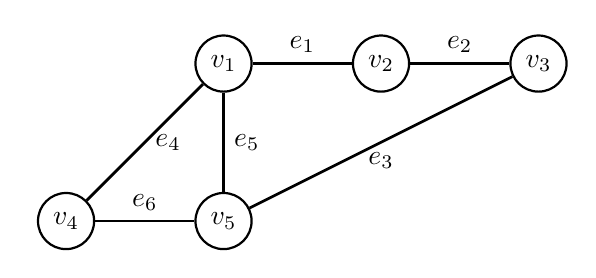
\begin{tikzpicture}
                    
                        \node[circle, draw, thick] (A) at (-1,2) {$v_1$};
                        \node[circle, draw, thick] (B) at (1,2) {$v_2$};
                        \node[circle, draw, thick] (C) at (3,2) {$v_3$};
                        \node[circle, draw, thick] (D) at (-3,0) {$v_4$};
                        \node[circle, draw, thick] (E) at (-1,0) {$v_5$};
      
                        \draw[line width=1pt] (A) -- node[midway, above] {$e_1$} (B);
                        \draw[line width=1pt] (A) -- node[midway, right] {$e_5$} (E);
                        \draw[line width=1pt] (A) -- node[midway, right] {$e_4$} (D);
                        \draw[line width=1pt] (B) -- node[midway, above] {$e_2$} (C);
                        \draw[line width=1pt] (C) -- node[midway, below] {$e_3$} (E);
                        \draw[line width=1pt] (D) -- node[midway, above] {$e_6$} (E);
    
                    \end{tikzpicture}

                \end{center}

            \end{ScientificDefinition}

            متن
        
\end{document}